\documentclass[aspectratio=169]{beamer}
\usepackage{will_handley_beamer}
\usepackage{title_page}

% Commands
% --------
% - \arxiv{arxiv number}
% - \arxiv{<number>}            arxiv.org/abs/<number>
% - \oldarxiv{<arxiv number>}   arxiv.org/<number>
% - \doi{<doi>}                 doi.org/<doi>
% - \xkcd{<number>}             xkcd.com/<number>
% - \email{<email>}             <<email>>
% - \tthref{<website>}          <website>
% - \av[dist]{<quantity>}       <quantity>_{dist}
% - \student{<name>}{<detail>}{<photo>}

% Talk details
% ------------
\title{Cosmological tensions?}
\subtitle{A guide for high energy theorists}
\date{1\textsuperscript{st} November 2024}

\begin{document}

\begin{frame}
    \titlepage
\end{frame}

\begin{frame}
    \frametitle{Structure}
    - Intro: what is the Hubble tension
    - Measurements and inference in cosmology
        - measuring distances is hard
            - standard candles
            - standard rulers
            - standard sirens
    - What is the Hubble constant
        - present day expansion rate of the universe
    - Challenges of 'measurement' in cosmology
        - difference with particle physics
    - frequentist vs bayesian inference in cosmology
        - frequentist approaches make sense in particle physics (independent identically distributed events)
        - in much of 
    - gotcha's
        - HEP and AP colour in their plots in opposite directions
        - marginalisation vs profiling
        - nuisance parameters
    - Plots:
        - H(z) with supernovae disagreeing
        - summary of all other measurements
    - Weak lensing tension
    - Curvature tension?
    - dark energy tension and DESI
    - Future
        - simulation-based inference
        - removing fiducial cosmology assumptions
        - lensed calibrators
    - Reference the upcoming tensions paper
\end{frame}

\begin{frame}
    \frametitle{<+Frame title+>}
    <+Content+>
\end{frame}

\begin{frame}
    \frametitle{Conclusions}
    \framesubtitle{\tthref{github.com/handley-lab}}
    \tikz[overlay,remember picture]
        \node[anchor=north east] (A) at ($(current page.north east)+(0,0)$) {
        
\includegraphics[width=0.10\textheight]{people/adam_ormondroyd.jpg}%
        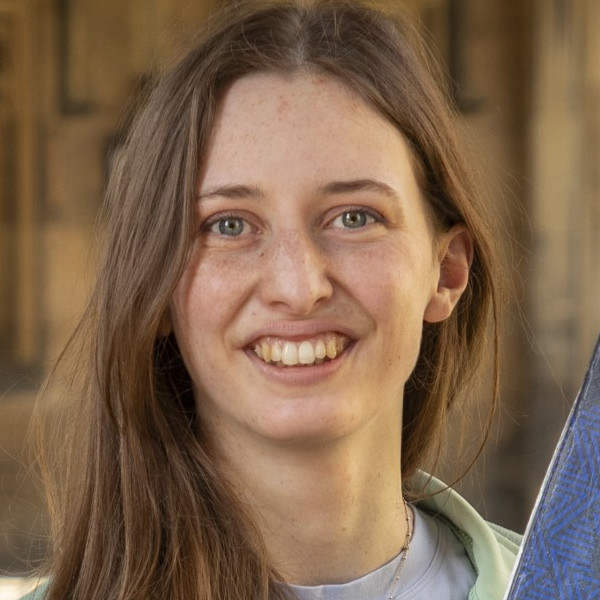
\includegraphics[width=0.10\textheight]{people/charlotte_priestley.jpg}%
        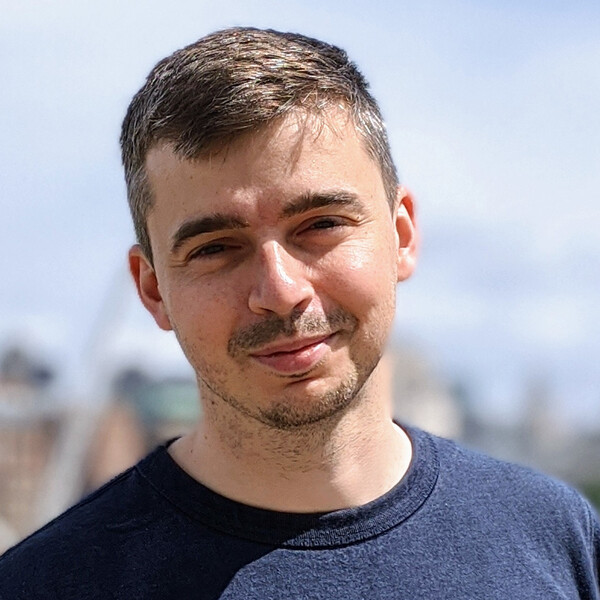
\includegraphics[width=0.10\textheight]{people/david_yallup.jpg}%
        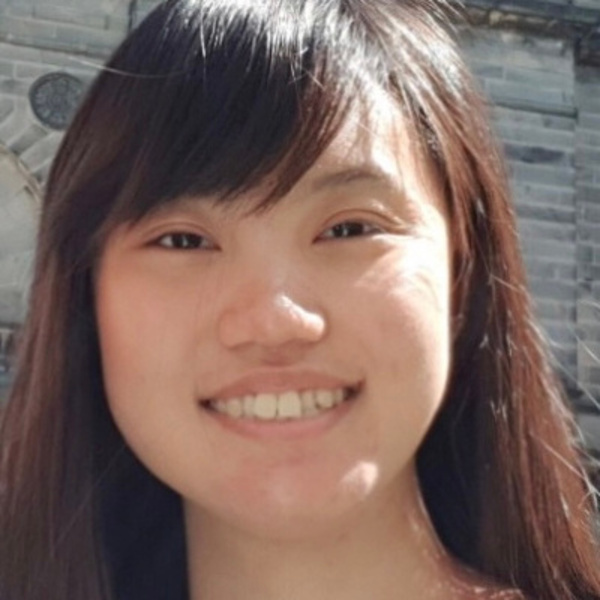
\includegraphics[width=0.10\textheight]{people/dily_ong.jpg}%
        
\includegraphics[width=0.10\textheight]{people/george_carter.jpg}%
        
\includegraphics[width=0.10\textheight]{people/harry_bevins.jpg}%
        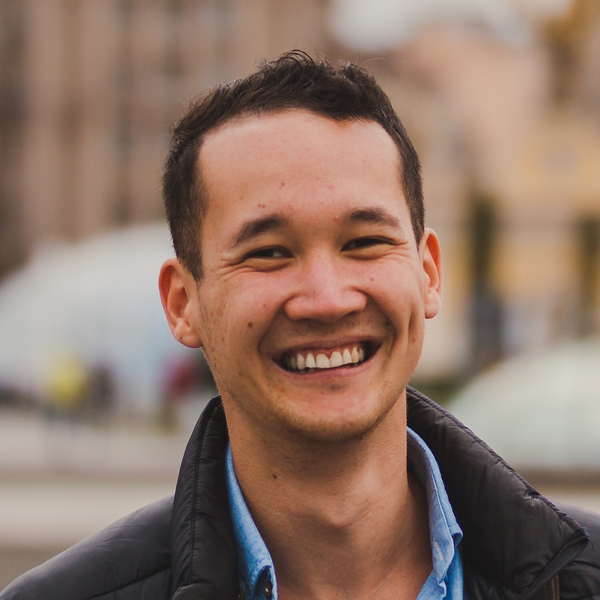
\includegraphics[width=0.10\textheight]{people/kilian_scheutwinkel.jpg}%
        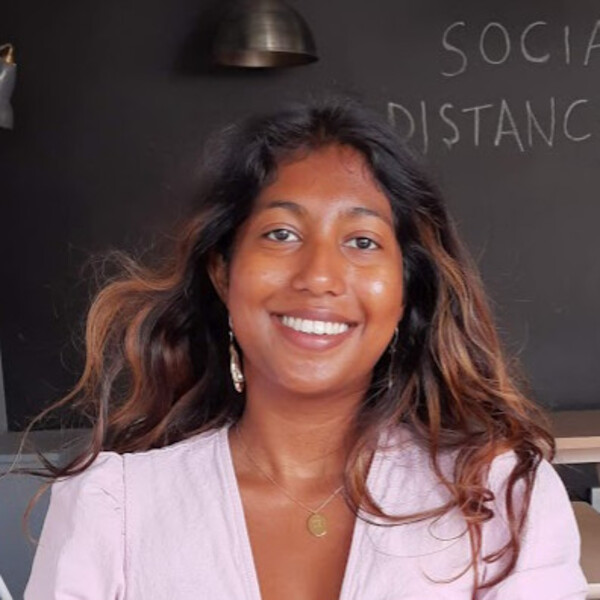
\includegraphics[width=0.10\textheight]{people/metha_prathaban.jpg}%
        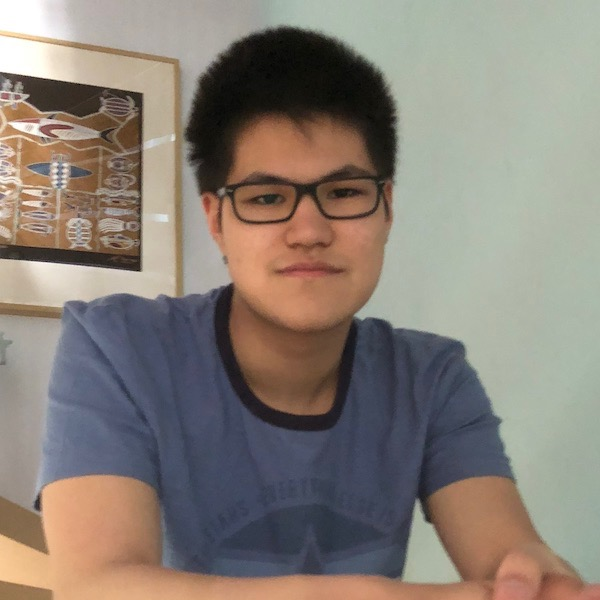
\includegraphics[width=0.10\textheight]{people/namu_kroupa.jpg}%
        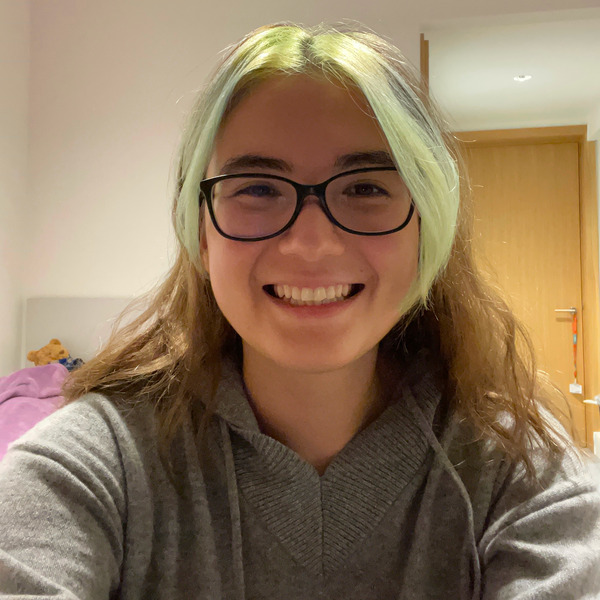
\includegraphics[width=0.10\textheight]{people/sinah_legner.jpg}%
        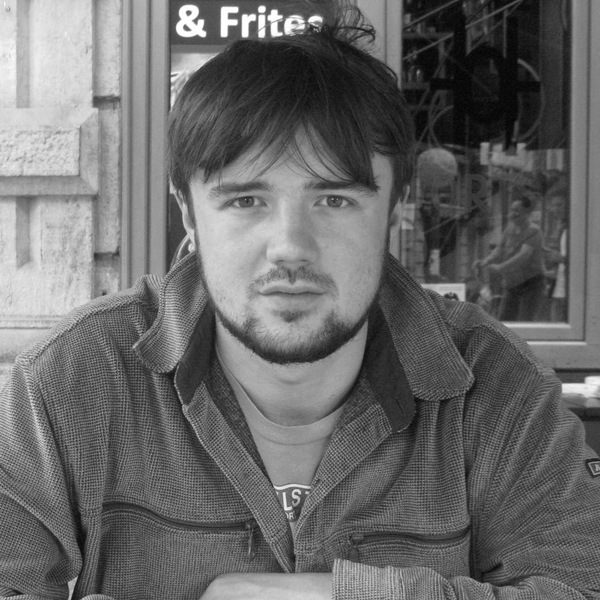
\includegraphics[width=0.10\textheight]{people/sam_leeney.jpg}%
        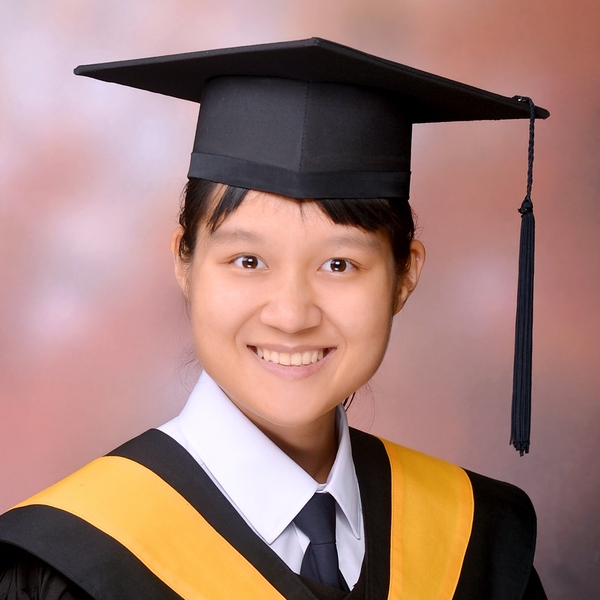
\includegraphics[width=0.10\textheight]{people/wei-ning_deng.jpg}%
        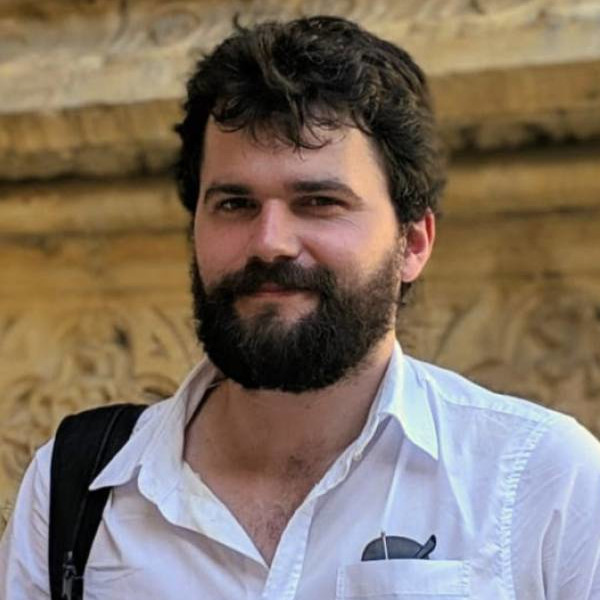
\includegraphics[width=0.10\textheight]{people/will_handley.jpg}%
    };
\end{frame}

\end{document}
